\section{Combination into a process-driven semi-event-based Micro-service DWS}
\label{sec:finalArchitecture}
After having introduced all the basic technologies this section aims to combine those into the process-driven semi-event-bases microservice architecture for Data Warehouse Systems. The focus will lie upon the interaction between multiple components and is quite generic. There will not be any detailed choice of various processes or products. In order to verify its usability and feasibility an evaluation from industrial point of view will be appended. This will be achieved by interviewing a technical expert.

\subsection{Introducing the Process-Driven Semi-Event-Based Microservice approach for Data Warehouse Systems}
\begin{figure}[!htb]
    \centering
    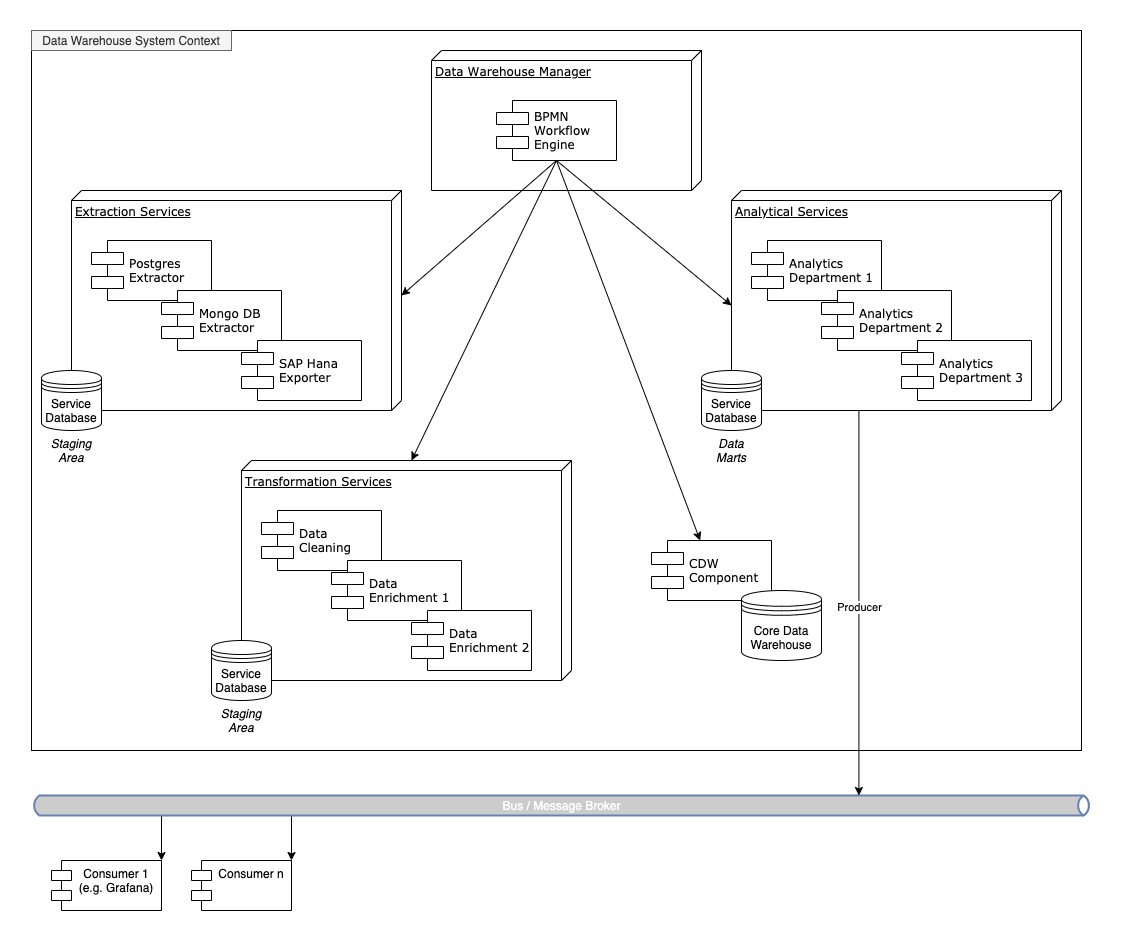
\includegraphics[scale=0.43]{pictures/ResultingArchitecture.png}
    \caption{Process-driven semi-event-bases microservice architecture for Data Warehouse Systems}
    \label{fig:resultingArch}
\end{figure}
Figure \ref{fig:resultingArch} shows the resulting architecture. In the next section we will have a more detailed summary of the components and their interactions.\newline
\\
Starting off with the Data Warehouse Manager, this component contains a BPMN workflow engine which is used for the orchestration of the whole system. Additionally all information of the process flow is stored and maintained within this component. \newline
Next up lets focus upon the service cluster for data extraction. It contains microservices as SCS which are controlled via the data warehouse manager. As shown in the diagram, each service has its own database. Typically for the extraction layer the staging area is used as temporal data storage.  It can be thought to have distinct services depending upon the input format. Nevertheless there are multiple other possibilities about how to split up this component. As mentioned within chapter \ref{sec:techKnowHow} it is empathised to slice the services along the process which is defined within the BPMN diagram.\newline
Besides of that the transformation services are orchestrated by the workflow engine as well. They get cascaded as needed within the BPMN diagrams. As shown in the cluster, data cleaning, cleansing and enhancement is provided. These self contained systems will hand over the data into a CDW component which stores the historical data.\newline
In the cluster for analytical services there are multiple instances which are used to extract and store a subset of data within data marts. Due to the orchestration done by BPM it is possible to cascade multiple services in order to make department specific analysis possible. Furthermore the information will be shared via a message broker or event bus system with various consumer which are often represented by departments. As shown within the picture it would be possible to use a Grafana or Tableau instance in order to generate reports from those information.\newline
\\
In conclusion the key features are contained within die SCS approach to DWS, the process driven orchestration using a BPMN workflow engine as well as the data supply via an event bus / message broker. By making use of these principle the overall systems gets more adaptive in terms of customer needs. The overall development and dependency management gets easier as well as faster. 

\subsection{Evaluation of this Architecture from an industrial Point of View}
\subsubsection{Design of Guidelines for Interview}
\subsubsection{Selection of proper Candidates}
\subsubsection{Resulting Feedback}
